% 第 1 章：集合与常用逻辑用语
% 对应第 1 章（1.1 集合、1.2 常用逻辑用语）
% 说明：本章按内容编排，课时划分由教师把握。
\section{集合与常用逻辑用语}

\begin{learnobjective}
\begin{itemize}
  \item 了解集合的含义，体会元素与集合之间的“属于”关系；
  \item 掌握列举法与描述法，能根据问题选择恰当的表示方法；
  \item 理解集合中元素的确定性、互异性与无序性；
  \item 会用集合的包含关系判断充分条件与必要条件。
\end{itemize}
\end{learnobjective}

\begin{preview}
\subsection*{知识回顾}
\begin{itemize}
  \item 自然数集记作 \blank，有理数集记作 \blank，实数集记作 \blank；
  \item 若 $a$ 是集合 $A$ 的元素，记作 \blank；否则记作 \blank。
\end{itemize}

\subsection*{课前速读}
阅读本章内容，完成下列问题：
\begin{enumerate}
  \item 集合中元素的三个特性是 \blank、\blank、\blank；
  \item 列举法的格式为 \blank；描述法的格式为 \blank；
  \item 设 $p$ 对应集合 $A$、$q$ 对应集合 $B$，则 $p$ 是 $q$ 的充分条件等价于 \blank。
\end{enumerate}
\end{preview}

\begin{explore}

\subsection{集合的含义与表示}

\key{探究一：集合的表示}
我们把研究对象统称为\key{元素}，把一些元素组成的总体叫做\key{集合}。
元素与集合的关系只有两种：$a\in A$ 或 $a\notin A$。

\begin{example}
用列举法表示集合 $\{x\in\mathbb{Z}\mid -2<x\le 3\}$。
\end{example}
\begin{solution}
逐一检验整数：$-1,0,1,2,3$，故为 $\{-1,0,1,2,3\}$。
\end{solution}

\key{探究二：描述法的代表元素}
比较 $\{x\mid x^2=1\}$、$\{y\mid y^2=1\}$、$\{(x,y)\mid x^2+y^2=1\}$ 三个集合。
\begin{solution}
前两个都是数集 $\{-1,1\}$，彼此相等；第三个是点集（单位圆），与前两个完全不同。
可见描述法中\key{代表元素与约束条件共同决定集合}。
\end{solution}

\key{探究三：元素与集合的关系}
\begin{problem}
已知 $A=\{1,a,a^2\}$，若 $2\in A$，求实数 $a$ 的值。
\end{problem}
\begin{solution}
若 $a=2$，则 $A=\{1,2,4\}$，符合；若 $a^2=2$，则 $a=\pm\sqrt{2}$，此时 $A=\{1,\pm\sqrt{2},2\}$，也符合。
故 $a=2$ 或 $a=\pm\sqrt{2}$。
\end{solution}

\key{探究四：集合中元素的三性}
\begin{problem}
集合 $\{1,1,2\}$ 能否表示一个集合？为什么？
\end{problem}
\begin{solution}
不能。集合中的元素必须\key{互异}，同一个元素只能出现一次，应写成 $\{1,2\}$。
\end{solution}

\subsection{充分条件与必要条件}

用集合的包含关系判断：设 $p$ 对应集合 $A$，$q$ 对应集合 $B$。
\begin{center}
\footnotesize
\setlength{\tabcolsep}{3pt}
\renewcommand{\arraystretch}{1.4}
\begin{tabular}{p{3.0cm}p{4.4cm}p{3.2cm}}
\toprule
集合关系 & 条件关系 & 记忆 \\
\midrule
$A=B$ & $p$ 是 $q$ 的充要条件 & 范围相等 \\
$A\subsetneqq B$ & $p$ 是 $q$ 的充分不必要条件 & 小推大 \\
$B\subsetneqq A$ & $p$ 是 $q$ 的必要不充分条件 & 大推小 \\
互不包含 & 既不充分也不必要 & 推不出 \\
\bottomrule
\end{tabular}
\end{center}

\begin{problem}
已知 $p$：$x\in(-1,3)$，$q$：$x^2-2x-3<0$。判断 $p$ 是 $q$ 的什么条件。
\end{problem}
\begin{solution}
$q$ 的解集为 $(-1,3)$，与 $p$ 的集合相同，即 $A=B$。
故 $p$ 是 $q$ 的充要条件。
\end{solution}

\begin{problem}
设 $p$：$x>3$，$q$：$x^2-2x-3>0$。判断 $p$ 是 $q$ 的什么条件。
\end{problem}
\begin{solution}
$q$ 的解集为 $(-\infty,-1)\cup(3,+\infty)$，$p$ 的集合 $(3,+\infty)$ 是其真子集，
故 $p$ 是 $q$ 的充分不必要条件。
\end{solution}

\begin{figure}[htbp]
  \centering
  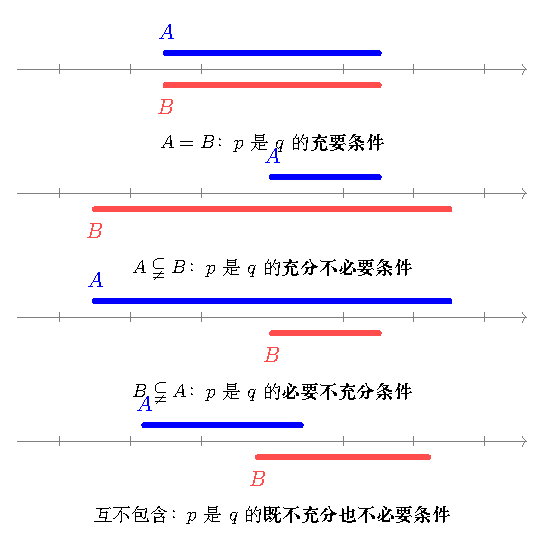
\includegraphics[width=0.70\textwidth]{set-conditions.pdf}
  \caption{四种条件关系的数轴表示}
\end{figure}

\key{一句话}：小范围推大范围，范围相等即充要。

\end{explore}

\begin{inclasstest}
\begin{enumerate}
  \item 下列对象能构成集合的是（　　）
  \begin{enumerate}[(A)]
    \item 很大的数；
    \item 我校高一年级全体女生；
    \item 好看的电视剧；
    \item 接近 $0$ 的实数。
  \end{enumerate}
  \item 用描述法表示集合 $\{1,3,5,7,9\}$：\blank。
  \item 设 $A=\{x\mid x<2\}$，$B=\{x\mid x<a\}$，若 $A\subseteq B$，则 $a$ 的取值范围是 \blank。
  \item 设 $p$：$x>3$，$q$：$x^2-2x-3>0$，判断 $p$ 是 $q$ 的什么条件。
\end{enumerate}
\end{inclasstest}

\begin{afterclass}
\begin{enumerate}
  \item 复习本章内容，完成课后练习；
  \item 思考题：集合 $\{x\mid x^2=a\}$ 在 $a<0$、$a=0$、$a>0$ 时分别表示什么？
  \item 设 $A=\{x\mid x^2-5x+6<0\}$，$B=\{x\mid 1<x<a\}$，若 $A\subseteq B$，求 $a$ 的取值范围。
\end{enumerate}
\reading{拓展阅读 01}{集合之美}
\end{afterclass}
